%==============================================================================
% Figure: Origami Folding Sequence (Dimensional Reduction)
% Purpose: Visual metaphor for dimensional compactification 8D -> 3D
% Chapter: Ch13 - Genesis Dimensional Structure
% Type: Conceptual
%==============================================================================

\begin{figure}[htbp]
  \centering
  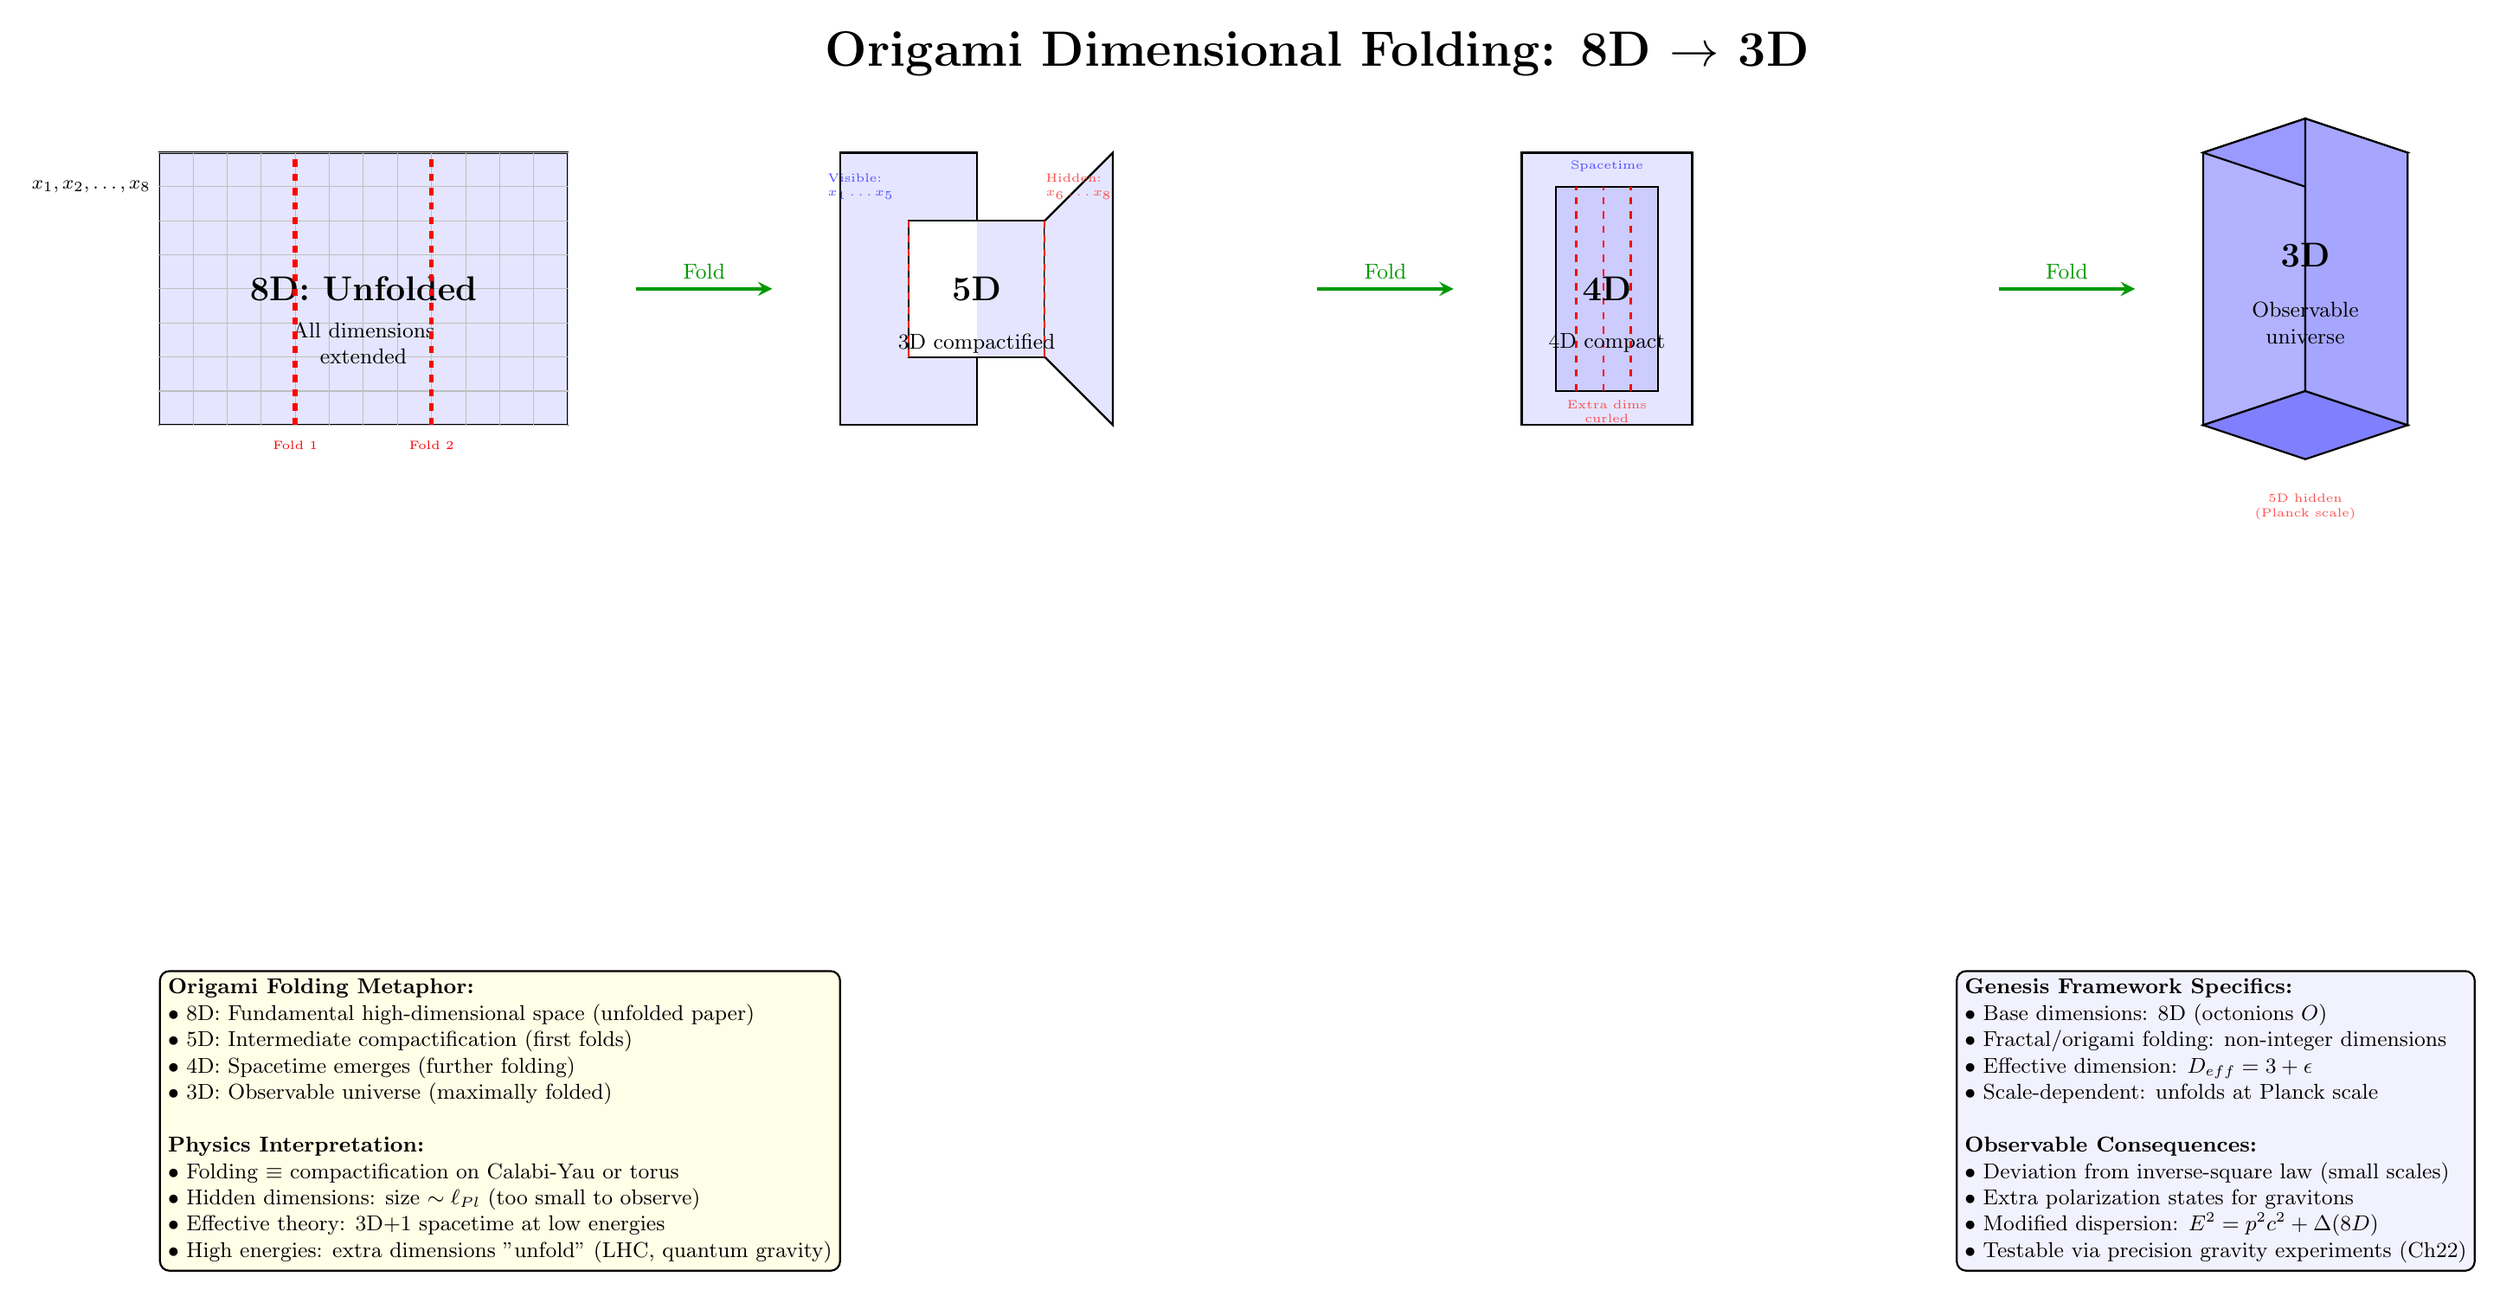
\begin{tikzpicture}[
    scale=1.0,
    paper/.style={fill=blue!10, draw=black, thick},
    fold/.style={thick, red, dashed},
    arrow/.style={ultra thick, ->, >=stealth, green!60!black}
  ]

    %========== Stage 1: 8D Unfolded (flat sheet) ==========
    \begin{scope}[shift={(0, 8)}]
      % Large flat rectangle representing unfolded 8D space
      \draw[paper] (0, 0) rectangle (6, 4);

      % Grid to show 8 dimensions symbolically
      \draw[thin, gray!50] (0, 0) grid[step=0.5] (6, 4);

      % Label
      \node[font=\Large\bfseries] at (3, 2) {8D: Unfolded};
      \node[font=\small, align=center] at (3, 1.2) {All dimensions\\extended};

      % Dimension labels
      \node[font=\footnotesize, left] at (0, 3.5) {$x_1, x_2, \ldots, x_8$};

      % Fold lines indicated
      \draw[fold, line width=2pt] (2, 0) -- (2, 4);
      \draw[fold, line width=2pt] (4, 0) -- (4, 4);
      \node[font=\tiny, text=red] at (2, -0.3) {Fold 1};
      \node[font=\tiny, text=red] at (4, -0.3) {Fold 2};
    \end{scope}

    % Arrow to next stage
    \draw[arrow] (7, 10) -- (9, 10) node[midway, above, font=\small] {Fold};

    %========== Stage 2: 5D Partially Folded ==========
    \begin{scope}[shift={(10, 8)}]
      % Folded shape (accordion-like)
      \draw[paper] (0, 0) -- (0, 4) -- (2, 4) -- (2, 3) -- (1, 3) -- (1, 1) -- (2, 1) -- (2, 0) -- cycle;
      \draw[paper] (2, 3) -- (3, 3) -- (3, 1) -- (2, 1);
      \draw[paper] (3, 3) -- (4, 4) -- (4, 0) -- (3, 1);

      % Indicate hidden dimensions
      \draw[fold] (1, 1) -- (1, 3);
      \draw[fold] (3, 1) -- (3, 3);

      % Label
      \node[font=\Large\bfseries] at (2, 2) {5D};
      \node[font=\small, align=center] at (2, 1.2) {3D compactified};

      % Dimension breakdown
      \node[font=\tiny, align=left, text=blue!70] at (0.3, 3.5) {Visible:\\$x_1 \ldots x_5$};
      \node[font=\tiny, align=left, text=red!70] at (3.5, 3.5) {Hidden:\\$x_6 \ldots x_8$};
    \end{scope}

    % Arrow to next stage
    \draw[arrow] (17, 10) -- (19, 10) node[midway, above, font=\small] {Fold};

    %========== Stage 3: 4D Further Folded ==========
    \begin{scope}[shift={(20, 8)}]
      % More compact folded shape
      \draw[paper] (0, 0) rectangle (2.5, 4);
      \draw[paper, fill=blue!20] (0.5, 0.5) rectangle (2, 3.5);

      % Interior folds
      \draw[fold] (0.8, 0.5) -- (0.8, 3.5);
      \draw[fold] (1.2, 0.5) -- (1.2, 3.5);
      \draw[fold] (1.6, 0.5) -- (1.6, 3.5);

      % Label
      \node[font=\Large\bfseries] at (1.25, 2) {4D};
      \node[font=\small, align=center] at (1.25, 1.2) {4D compact};

      % Annotations
      \node[font=\tiny, text=blue!70] at (1.25, 3.8) {Spacetime};
      \node[font=\tiny, text=red!70, align=center] at (1.25, 0.2) {Extra dims\\curled};
    \end{scope}

    % Arrow to final stage
    \draw[arrow] (27, 10) -- (29, 10) node[midway, above, font=\small] {Fold};

    %========== Stage 4: 3D Maximally Folded ==========
    \begin{scope}[shift={(30, 8)}]
      % Small compact cube (projected)
      \draw[paper, fill=blue!30] (0, 0) -- (1.5, 0.5) -- (1.5, 4.5) -- (0, 4) -- cycle;
      \draw[paper, fill=blue!40] (0, 4) -- (1.5, 4.5) -- (3, 4) -- (1.5, 3.5) -- cycle;
      \draw[paper, fill=blue!50] (0, 0) -- (1.5, 0.5) -- (3, 0) -- (1.5, -0.5) -- cycle;
      \draw[paper, fill=blue!35] (3, 0) -- (3, 4) -- (1.5, 4.5) -- (1.5, 0.5) -- cycle;

      % Label
      \node[font=\Large\bfseries] at (1.5, 2.5) {3D};
      \node[font=\small, align=center] at (1.5, 1.5) {Observable\\universe};

      % Compactified dimensions
      \node[font=\tiny, text=red!70, align=center] at (1.5, -1.2) {5D hidden\\(Planck scale)};
    \end{scope}

    %========== Bottom: Explanation ==========
    \begin{scope}[shift={(0, 0)}]
      \node[anchor=north west, align=left, font=\small, draw=black, fill=yellow!10, rounded corners, thick]
        at (0, 0) {
        \textbf{Origami Folding Metaphor:} \\
        $\bullet$ 8D: Fundamental high-dimensional space (unfolded paper) \\
        $\bullet$ 5D: Intermediate compactification (first folds) \\
        $\bullet$ 4D: Spacetime emerges (further folding) \\
        $\bullet$ 3D: Observable universe (maximally folded) \\
        \\
        \textbf{Physics Interpretation:} \\
        $\bullet$ Folding $\equiv$ compactification on Calabi-Yau or torus \\
        $\bullet$ Hidden dimensions: size $\sim \ell_{\text{Pl}}$ (too small to observe) \\
        $\bullet$ Effective theory: 3D+1 spacetime at low energies \\
        $\bullet$ High energies: extra dimensions "unfold" (LHC, quantum gravity)
      };

      \node[anchor=north east, align=left, font=\small, draw=black, fill=blue!5, rounded corners, thick]
        at (34, 0) {
        \textbf{Genesis Framework Specifics:} \\
        $\bullet$ Base dimensions: 8D (octonions $\mathbb{O}$) \\
        $\bullet$ Fractal/origami folding: non-integer dimensions \\
        $\bullet$ Effective dimension: $D_{\text{eff}} = 3 + \epsilon$ \\
        $\bullet$ Scale-dependent: unfolds at Planck scale \\
        \\
        \textbf{Observable Consequences:} \\
        $\bullet$ Deviation from inverse-square law (small scales) \\
        $\bullet$ Extra polarization states for gravitons \\
        $\bullet$ Modified dispersion: $E^2 = p^2c^2 + \Delta(8D)$ \\
        $\bullet$ Testable via precision gravity experiments (Ch22)
      };
    \end{scope}

    % Title
    \node[anchor=south, font=\huge\bfseries] at (17, 13) {Origami Dimensional Folding: 8D $\to$ 3D};

  \end{tikzpicture}
  \caption{Visual metaphor for dimensional compactification in the Genesis framework using origami
    folding. The sequence shows the progression from an unfolded 8-dimensional space (flat sheet
    with grid) through intermediate stages (5D, 4D with progressive folding) to the final maximally
    folded 3D observable universe (compact cube). Red dashed lines indicate fold boundaries where
    dimensions become compactified. The origami analogy captures key physics: just as folding paper
    reduces its apparent dimensionality while preserving the full structure, compactification hides
    extra spatial dimensions at the Planck scale ($\sim 10^{-35}$ m) while maintaining their
    influence on high-energy physics. The Genesis framework starts with 8 fundamental dimensions
    (tied to octonion algebra $\mathbb{O}$) and employs fractal/origami folding to produce an
    effective dimension $D_{\text{eff}} = 3 + \epsilon$, slightly above 3. This predicts observable
    deviations from inverse-square gravity at small scales and modified dispersion relations,
    testable in precision experiments (Ch22). At high energies (approaching Planck scale), the
    folded dimensions "unfold," revealing the full 8D structure.}
  \label{fig:origami-folding-sequence}
\end{figure}
